\label{Containers_Azure}
\section{Creation of Microsoft Azure \acrshort{vm}}
\begin{figure}[h]
	\begin{subfigure}{\textwidth}
		\captionsetup{width=0.9\linewidth}
		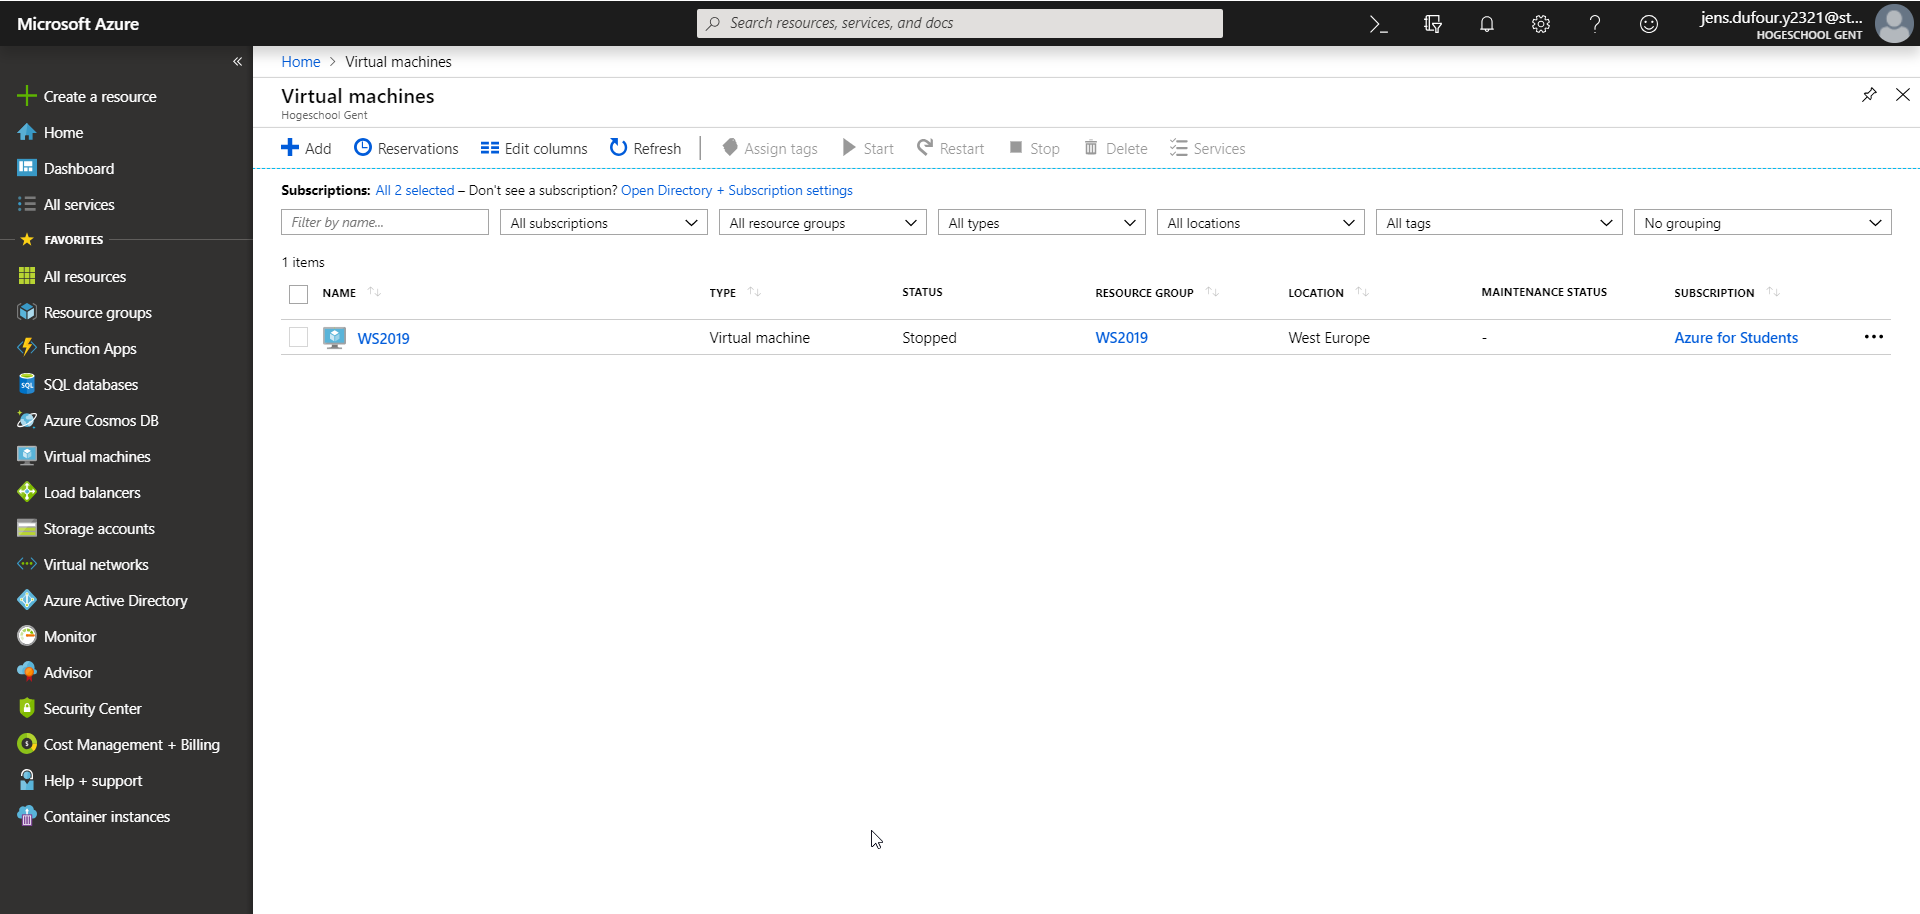
\includegraphics[width=\linewidth]{img/Container_VM_0.png} 
		\centering
		\caption{Add a new \acrshort{vm} through the Azure Portal}
		\label{fig:Container_VM_0}
	\end{subfigure}
\end{figure}
\begin{figure}[h]\ContinuedFloat
	\begin{subfigure}{\textwidth}
		\captionsetup{width=0.9\linewidth}
		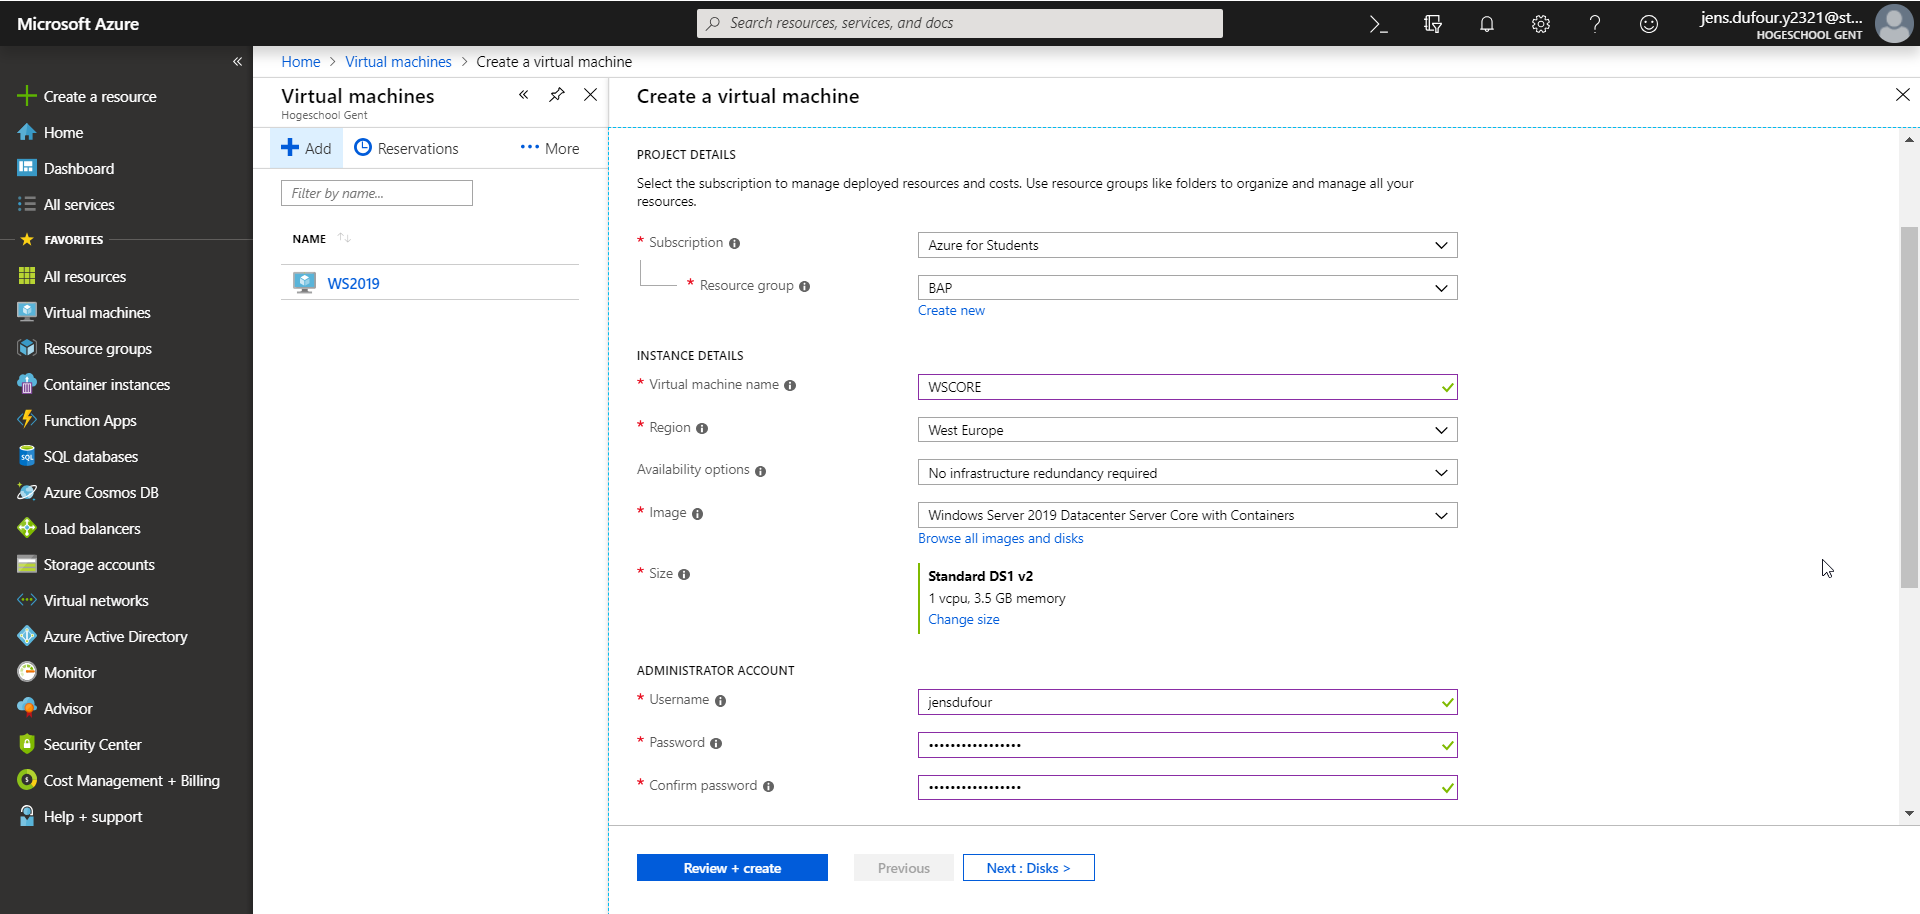
\includegraphics[width=\linewidth]{img/Container_VM_1.png}
		\centering
		\caption{Fill in the required parameters and select the correct image}
		\label{fig:Container_VM_1}
	\end{subfigure}
\end{figure}
\begin{figure}[h]\ContinuedFloat
	\begin{subfigure}{\textwidth}
		\captionsetup{width=0.9\linewidth}
		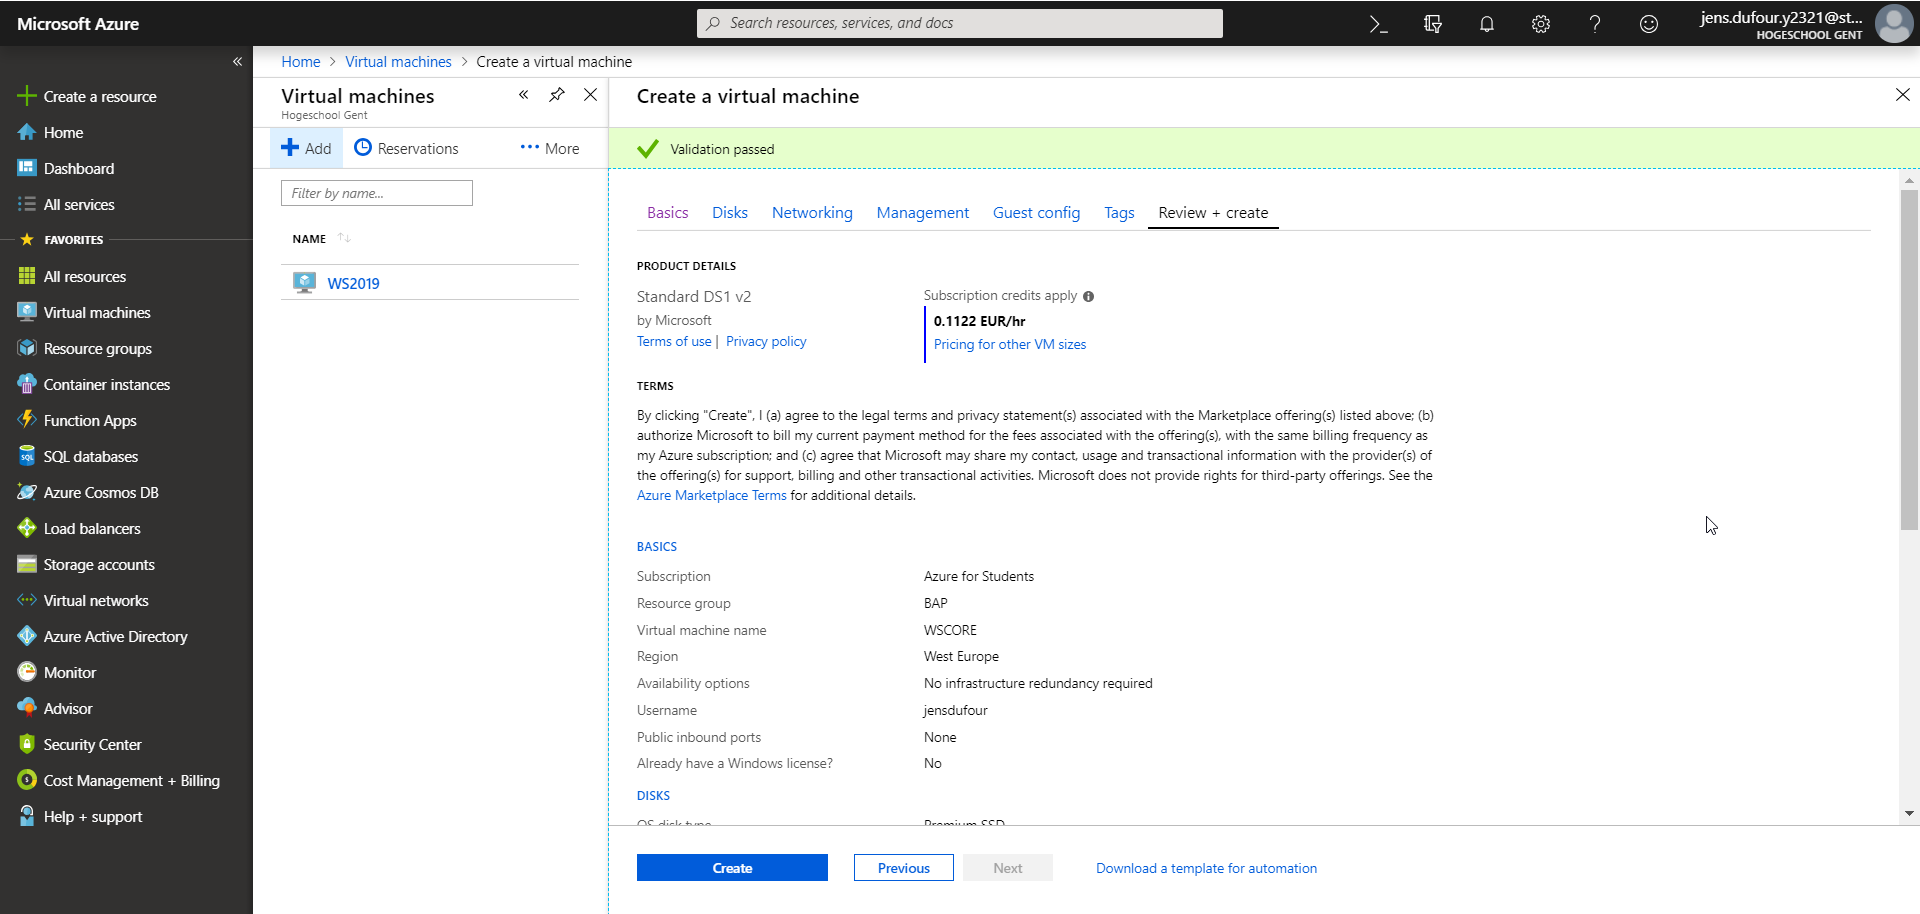
\includegraphics[width=\linewidth]{img/Container_VM_2.png}
		\centering
		\caption{Review the parameters and create the \acrshort{vm}}
		\label{fig:Container_VM_2}
	\end{subfigure}
	\caption{Creation of Microsoft Azure \acrshort{vm}}
	\label{fig:Container_VM}
\end{figure}
\clearpage
\section{Installation of nested \acrshort{vm}}
The following commands have to be run through Powershell on the created \acrshort{vm} to install the requirements needed to run a nested \acrshort{vm}. This is necessary to run the containers isolated.
\begin{lstlisting}[breaklines]
Install-WindowsFeature -Name Hyper-V
Install-WindowsFeature -Name Containers
Enable-WindowsOptionalFeature -Online -FeatureName Microsoft-Hyper-V -All
Enable-WindowsOptionalFeature -Online -FeatureName containers -All
\end{lstlisting}
\section{Installation of Git}
The following commands have to be run through Powershell on the created \acrshort{vm} to install Git. Git is necessary to clone the files needed to run the benchmarks.
\begin{lstlisting}[breaklines]
Set-ExecutionPolicy Bypass -Scope Process -Force;iex ((New-Object System.Net.WebClient).DownloadString('https://chocolatey.org/install.ps1'))
choco install git -params '"/GitAndUnixToolsOnPath"' -y
refreshenv
\end{lstlisting}
\section{Installation of Docker EE}
The following commands have to be run through Powershell on the created \acrshort{vm} to install Docker EE.
\begin{lstlisting}[breaklines]
Install-Module -Name DockerMsftProvider -Repository PSGallery -Force
Install-Package -Name docker -ProviderName DockerMsftProvider
Restart-Computer -Force
\end{lstlisting}